\documentclass[journal,onecolumn]{IEEEtran}
\usepackage{cite}
\usepackage{amsmath,amssymb}
\usepackage{graphicx}
\usepackage{booktabs}
\usepackage{multirow}
\usepackage{array}
\usepackage{url}
\usepackage[hidelinks]{hyperref}
\graphicspath{{figures/}}
\renewcommand{\thetable}{S\arabic{table}}
\renewcommand{\thefigure}{S\arabic{figure}}
\begin{document}
\title{Supplementary Material for ``Leakage-Aware, Sensitivity-First Validation of Blood-Smear Leukemia Classifiers: A Two-Dataset Study of Engineered Features, Deep Features and Dimensionality Reduction''}
\author{First~Author and Second~Author}
\maketitle
\noindent This document contains the complete settings, computing environment, full parameter sweeps and secondary analyses referred to in the main text. Code, split files and per-model outputs are released with the paper.

\section*{S1. Settings and computing environment}
\begin{table*}[!t]
\centering
\caption{Complete settings of every component. All values were fixed in advance or taken from library defaults; none was fitted or tuned on an external set. Defaults of the named libraries apply to anything not listed.}
\label{tab:hparams}
\setlength{\tabcolsep}{4pt}
\renewcommand{\arraystretch}{1.05}
\footnotesize
\begin{tabular}{p{3.0cm}p{5.6cm}p{8.3cm}}
\toprule
Component & Setting & Value \\
\midrule
\multirow{5}{3.0cm}{Data and splits} & Development / external cohorts & APL-AML: Discovery (82 patients) / Validation (24 patients), split by diagnosis date by the data owners \\
 & Second dataset & C-NMC 2019: official folds 0--1 (42 subjects) / fold 2 (31 subjects), designated before any analysis \\
 & Cross-validation & 5 folds; image-level \texttt{StratifiedKFold} or patient-level \texttt{StratifiedGroupKFold} (cells), \texttt{StratifiedKFold} over patients (T3) \\
 & Random seeds & 0, 1, 2 (fold assignment, cell sampling, model initialization); results are averaged over seeds \\
 & Cells per patient (T3) & Up to 500, sampled at random once (seed 0); patients with fewer cells keep all \\
\midrule
\multirow{7}{3.0cm}{Engineered features (93)} & Input & RGB, bilinear resize to $192\times192$ \\
 & Color deconvolution & Ruifrok--Johnston H\&E matrix (\texttt{skimage rgb2hed}) \\
 & Nucleus & Gaussian smoothing ($\sigma=1$) of hematoxylin, Otsu threshold, opening (disk 2), component nearest the center (within $0.30\times$ image size); fallback: darkest 15\% of gray levels \\
 & Cytoplasm proxies & Basophilic region: blue-dominant pixels within one nuclear radius, opening (disk 2), closing (disk 4); ring: 2--9 px from the nucleus, excluding pixels brighter than the 90th lightness percentile $-3$ \\
 & Texture & GLCM on 33 gray levels, distances 1, 2, 4 px, angles $0,\pi/4,\pi/2,3\pi/4$ (contrast, dissimilarity, homogeneity, energy, correlation; averaged over angles); uniform LBP with $(P,R)=(8,1)$ and $(16,2)$ \\
 & Missing values & Unreadable images give NaN rows, imputed with the training-fold median \\
 & C-NMC background & Pixels with brightest channel $<15$ set to white before feature extraction (engineered features only) \\
\midrule
\multirow{3}{3.0cm}{Deep features} & Encoder & EfficientNet-B0, ImageNet weights (\texttt{timm}), frozen, global-average-pooled 1,280-d output \\
 & Input & Bicubic resize to $224\times224$, ImageNet mean/std normalization, no augmentation \\
 & Extraction & Batch size 64, 2 data-loader workers, CPU, \texttt{torch.no\_grad} \\
\midrule
\multirow{3}{3.0cm}{Feature engineering} & PCA & Standardization then PCA (\texttt{svd\_solver}=auto, \texttt{random\_state}=0), both fitted on training-fold cells only; 16, 32, 64 components pre-specified; 4, 8, 128, 256 as sensitivity analysis; pooled component statistics divided by one common scale (no whitening); per-component standardization reported for comparison \\
 & Correlation filter & Drop the later feature of every pair with $|r|>0.9$ (training cells, $\le$20,000 sampled) \\
 & Stain normalization / L1 & Per-slide median/SD standardization of the 26 stain features; L1-penalized LR, $C=0.5$, SAGA solver \\
\midrule
\multirow{3}{3.0cm}{Cell-level classifiers (T1, T2)} & Logistic regression & L2, $C=0.1$, L-BFGS, 3,000 iterations, class-balanced weights; median imputation and standardization inside the pipeline \\
 & LightGBM & 400 trees, learning rate 0.05, 31 leaves, row subsampling 0.8 (every iteration), column subsampling 0.8, class-balanced weights, 2 threads \\
 & Calibration & Temperature scaling fitted on an inner 80/20 split of the training fold (bounded search 0.05--20) \\
\midrule
\multirow{2}{3.0cm}{Pooled patient model (T3)} & Patient vector & Mean, SD, 10th, 50th, 90th percentile of every cell feature ($5\times$ dimensions) \\
 & Classifier & LR, L2, $C=0.1$, 5,000 iterations, class-balanced weights, standardization inside the pipeline \\
\midrule
\multirow{5}{3.0cm}{Gated attention MIL (T3)} & Architecture & Linear($d\to128$)--ReLU--Dropout(0.25); gated attention with $\tanh$ and sigmoid branches of 64 units; linear classifier on the attention-weighted mean \\
 & Optimization & AdamW, learning rate $2\times10^{-4}$ (constant, no schedule), weight decay $10^{-3}$, one bag per step, 40 epochs, no early stopping \\
 & Loss & Binary cross-entropy with positive-class weight $n_{\mathrm{AML}}/n_{\mathrm{APL}}$ of the training fold \\
 & Augmentation & Random removal of 20\% of a bag's cells at every step (bags with more than 10 cells) \\
 & Input scaling & Median imputation and standardization from training-fold cells \\
\midrule
\multirow{4}{3.0cm}{Fine-tuned CNN (T1, T2)} & Trainable part & EfficientNet-B0 stages 6--7, $1\times1$ head convolution (1,280 channels), new linear classifier (dropout 0.2); stem and stages 1--5 frozen, their $112\times14\times14$ outputs cached once (float16) \\
 & Optimization & AdamW, peak learning rate $3\times10^{-4}$, 1 warm-up epoch then cosine decay, weight decay $10^{-4}$, batch 128, 6 epochs, class-weighted binary cross-entropy \\
 & Data & Up to 5,000 training cells per fold (random); 15\% of training patients (grouped split) or images (image split) as inner validation for early stopping by validation loss; one seed \\
 & Augmentation & Random horizontal and vertical flips and $90^{\circ}$ rotations of the cached feature maps \\
\midrule
\multirow{2}{3.0cm}{Re-run baselines} & B1, B2 & Promyelocyte fraction (ranked directly); LR on the 17-class differential count \\
 & B3 & EfficientNet-B0 + RBF-SVM ($C=1$, $\gamma$ = \texttt{scale}, Platt probabilities, class-balanced, 8,000 training cells), cell scores averaged per patient \\
\midrule
\multirow{5}{3.0cm}{Operating point and statistics} & Threshold & Highest threshold giving sensitivity $\ge0.95$ on out-of-fold Discovery predictions; Youden threshold reported for reference \\
 & External prediction (T3) & Mean of the 15 fold models (5 folds $\times$ 3 seeds) \\
 & Confidence intervals & Patient-level bootstrap, 2,000 resamples (1,000 for cell-level CV); paired differences 4,000 resamples \\
 & Calibration error & ECE with 15 equal-width bins \\
 & Multiplicity & Holm correction across the comparisons reported in a table \\
\midrule
\multirow{3}{3.0cm}{Additional analyses} & Pooled CV (APL-AML) & 3 repeats $\times$ 5-fold patient CV over all 106 patients, stratified by diagnosis and cohort; threshold from an inner 3-fold CV \\
 & Local recalibration & $k\in\{2,4,6,8\}$ local Validation patients ($k/2$ per class), 2,000 draws; threshold lowered to just below the lowest local APL score \\
 & Decision curves & Platt recalibration on Discovery out-of-fold scores, prior shift to 10\% prevalence, threshold probabilities 0.01--0.60 \\
\bottomrule
\end{tabular}
\end{table*}

\begin{table}[!htbp]
\centering
\caption{Computing environment and run times.}
\label{tab:env}
\resizebox{\columnwidth}{!}{%
\begin{tabular}{ll}
\toprule
Item & Specification \\
\midrule
Hardware & Intel Xeon 2.80\,GHz, 2 vCPUs, 7.8\,GB RAM, no GPU \\
Software & Ubuntu 24.04.5 LTS; Python 3.13.16; PyTorch 2.14.1 (CPU); \\
 & scikit-learn 1.9.1 \cite{pedregosa2011sklearn}; LightGBM 4.7.0; scikit-image 0.26.0; timm 1.0.30 \\
Random seeds & 0, 1, 2 \\
Engineered features & 16.1\,min for 25,724 cells (2 processes) \\
EfficientNet-B0 embeddings & 51.2\,min for 25,724 cells (2 threads) \\
Cell-level model, 5-fold CV & 11--40\,s (LR), 15--600\,s (LightGBM) \\
Attention MIL, 5-fold CV & 33--61\,s per seed \\
\bottomrule
\end{tabular}}
\end{table}

\section*{S2. Evaluation protocols and segmentation}
\begin{figure}[!htbp]
\centering
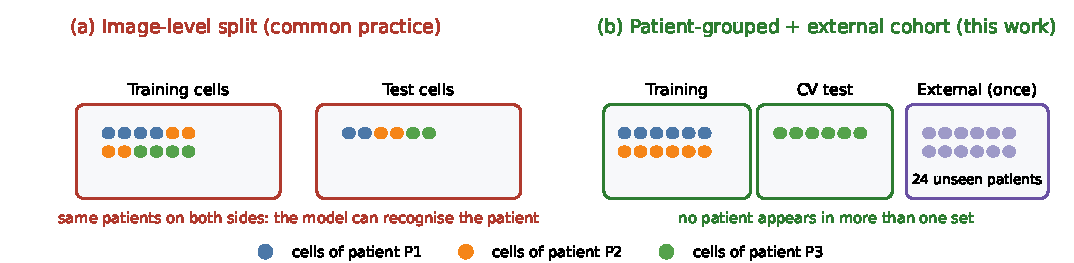
\includegraphics[width=\textwidth]{fig_splits.pdf}
\caption{Evaluation protocols. (a) Image-level splitting places cells of the same patient in training and test sets. (b) Patient-grouped splitting with an external cohort, used in this work; the external cohort is scored once.}
\label{fig:splits}
\end{figure}
\begin{figure}[!htbp]
\centering
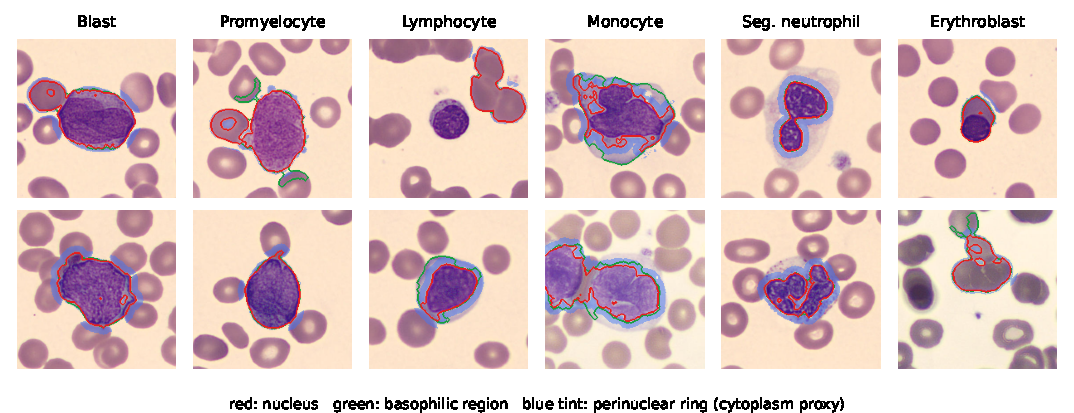
\includegraphics[width=\textwidth]{fig_segmentation.pdf}
\caption{Segmentation behind the engineered features, shown on cells at the 25th and 75th percentile of each class list. Red: nucleus; green: basophilic region; blue tint: perinuclear ring. The upper lymphocyte and lower erythroblast illustrate failures in which the mask falls on neighboring red cells.}
\label{fig:seg}
\end{figure}

\section*{S3. Feature engineering and full PCA sweep}
\begin{table*}[!t]
\centering
\caption{Feature engineering for patient-level APL detection. All steps are fitted inside the Discovery training folds; the Validation cohort is scored once. $\Delta$: external AUROC change relative to the unreduced representation (paired patient bootstrap). The configuration with the highest Discovery CV AUROC (pre-declared selection rule) is marked $^{\star}$. Oracle column: specificity at 100\% recall if the threshold were re-set on the Validation cohort (reference only, not deployable).}
\label{tab:fe}
\setlength{\tabcolsep}{3pt}
\resizebox{\textwidth}{!}{%
\begin{tabular}{llccccccc}
\toprule
Representation & Engineering step & CV AUROC & External AUROC [95\% CI] & $\Delta$ [95\% CI] & Recall (missed) & Spec. & F1 & Oracle spec. \\
\midrule
Engineered, all 93 & -- & 0.926 & 0.729 [0.511, 0.924] & -- & 0.58 (5/12) & 0.67 & 0.61 & 0.33 \\
Engineered & Correlation filter ($|r|>0.9$) & 0.922 & 0.736 [0.529, 0.930] & +0.007 [-0.070, +0.084] & 0.58 (5/12) & 0.67 & 0.61 & 0.42 \\
Engineered & Per-slide stain normalization & 0.872 & 0.576 [0.329, 0.818] & -0.153 [-0.326, +0.021] & 0.67 (4/12) & 0.50 & 0.62 & 0.08 \\
Engineered & L1 (LASSO) selection & 0.898 & 0.590 [0.350, 0.820] & -0.139 [-0.274, -0.023]* & 0.75 (3/12) & 0.42 & 0.64 & 0.17 \\
Engineered & Filter + stain normalization & 0.869 & 0.569 [0.322, 0.798] & -0.160 [-0.333, +0.009] & 0.67 (4/12) & 0.50 & 0.62 & 0.08 \\
\midrule
EfficientNet-B0, 1,280-d & -- & 0.957 & 0.743 [0.538, 0.926] & -- & 0.50 (6/12) & 0.67 & 0.55 & 0.42 \\
EfficientNet-B0 & PCA, 16 components & 0.909 & 0.792 [0.580, 0.963] & +0.049 [-0.096, +0.213] & 0.92 (1/12) & 0.67 & 0.81 & 0.42 \\
EfficientNet-B0 & PCA, 32 components & 0.958 & 0.833 [0.644, 0.972] & +0.090 [-0.014, +0.210] & 0.50 (6/12) & 0.92 & 0.63 & 0.42 \\
EfficientNet-B0$^{\star}$ & PCA, 64 components & 0.966 & 0.819 [0.604, 1.000] & +0.076 [-0.171, +0.324] & 0.50 (6/12) & 0.92 & 0.63 & 0.00 \\
\midrule
Fusion & Filter + PCA-32 & 0.960 & 0.764 [0.566, 0.938] & +0.021 [-0.105, +0.140] & 0.58 (5/12) & 0.83 & 0.67 & 0.42 \\
Digital differential & 8 predicted cell classes & 0.852 & 0.785 [0.570, 0.953] & +0.056 [-0.104, +0.229] & 1.00 (0/12) & 0.33 & 0.75 & 0.50 \\
Differential + engineered & Filtered & 0.928 & 0.764 [0.562, 0.943] & +0.035 [-0.015, +0.111] & 0.58 (5/12) & 0.67 & 0.61 & 0.50 \\
Engineered, attention MIL & Filter + stain normalization & 0.922 & 0.569 [0.326, 0.793] & -0.160 [-0.422, +0.091] & 0.42 (7/12) & 0.75 & 0.50 & 0.17 \\
EfficientNet-B0, attention MIL & PCA-32 & 0.924 & 0.799 [0.580, 0.972] & +0.069 [-0.133, +0.281] & 0.50 (6/12) & 0.75 & 0.57 & 0.50 \\
\bottomrule
\multicolumn{9}{l}{\footnotesize Recall, specificity and F1 at the operating point fixed on Discovery (target sensitivity 0.95). * $p<0.05$ unadjusted; $^{\dagger}$ $p<0.05$ after Holm correction across all comparisons in the table.}
\end{tabular}}
\end{table*}
\begin{table*}[!t]
\centering
\caption{Patient/subject-level detection before and after PCA of the EfficientNet-B0 embeddings (pooled-statistics LR), on both datasets. PCA is fitted on training-fold cells only; the principal-component scores keep their relative variances (no whitening). Std.: external AUROC when each component is instead standardized to unit variance before the classifier (whitening), as in our first analysis. $\Delta$: change in external AUROC relative to no PCA under the same scaling (paired bootstrap). Recall, specificity at the operating point fixed on development data. Components 16, 32 and 64 were pre-specified.}
\label{tab:pca}
\setlength{\tabcolsep}{2.6pt}
\resizebox{\textwidth}{!}{%
\begin{tabular}{rcccccccccccc}
\toprule
 & \multicolumn{6}{c}{APL-AML (24 external patients, 12 APL)} & \multicolumn{6}{c}{C-NMC (31 external subjects, 17 ALL)} \\
\cmidrule(lr){2-7}\cmidrule(lr){8-13}
Components & Var. & Std. & External [95\% CI] & $\Delta$ & Recall (missed) & Spec. & Var. & Std. & External [95\% CI] & $\Delta$ & Recall (missed) & Spec. \\
\midrule
None (1,280) & 1.00 & 0.743 & 0.708 [0.493, 0.907] & -- & 0.67 (4/12) & 0.67 & 1.00 & 0.908 & 0.908 [0.786, 0.992] & -- & 1.00 (0/17) & 0.64 \\
\midrule
8 & 0.35 & 0.674 & 0.646 [0.412, 0.860] & -0.062 & 0.33 (8/12) & 0.75 & 0.47 & 0.849 & 0.803 [0.637, 0.934] & -0.105* & 0.88 (2/17) & 0.36 \\
16 & 0.45 & 0.792 & 0.715 [0.496, 0.907] & +0.007 & 0.50 (6/12) & 0.75 & 0.58 & 0.798 & 0.819 [0.657, 0.949] & -0.088* & 0.94 (1/17) & 0.36 \\
32 & 0.55 & 0.833 & 0.785 [0.580, 0.950] & +0.076 & 0.50 (6/12) & 0.75 & 0.67 & 0.790 & 0.840 [0.689, 0.958] & -0.067 & 0.94 (1/17) & 0.43 \\
64 & 0.64 & 0.819 & 0.792 [0.594, 0.957] & +0.083 & 0.50 (6/12) & 0.75 & 0.76 & 0.739 & 0.853 [0.705, 0.965] & -0.055 & 0.94 (1/17) & 0.50 \\
128 & 0.73 & 0.646 & 0.778 [0.586, 0.950] & +0.069 & 0.50 (6/12) & 0.75 & 0.84 & 0.676 & 0.866 [0.726, 0.971] & -0.042 & 1.00 (0/17) & 0.50 \\
256 & 0.83 & 0.743 & 0.778 [0.586, 0.950] & +0.069 & 0.50 (6/12) & 0.75 & 0.91 & 0.655 & 0.870 [0.732, 0.974] & -0.038 & 1.00 (0/17) & 0.50 \\
\bottomrule
\multicolumn{13}{l}{\footnotesize Var.: cumulative explained variance on development cells. * $p<0.05$ unadjusted; $^{\dagger}$ $p<0.05$ after Holm correction.}
\end{tabular}}
\end{table*}

\section*{S4. Training settings and learning curves}
\begin{table}[!t]
\centering
\caption{Attention MIL trained for a fixed 40 epochs or with the number of epochs chosen by nested 3-fold CV inside each training fold (lowest mean validation loss). External AUROC, recall, F1 and calibration error (ECE); SD: spread of development CV AUROC across seeds.}
\label{tab:epochs}
\setlength{\tabcolsep}{2.2pt}
\resizebox{\columnwidth}{!}{%
\begin{tabular}{llccccccc}
\toprule
 & & \multicolumn{2}{c}{External AUROC} & \multicolumn{2}{c}{F1} & \multicolumn{2}{c}{ECE} & Chosen epochs \\
\cmidrule(lr){3-4}\cmidrule(lr){5-6}\cmidrule(lr){7-8}
Dataset & Features & Fixed & Nested & Fixed & Nested & Fixed & Nested & median (range) \\
\midrule
APL-AML & Engineered & 0.812 & 0.819 & 0.67 & 0.67 & 0.26 & 0.26 & 18 (3--37) \\
 & EfficientNet-B0 & 0.674 & 0.667 & 0.55 & 0.57 & 0.36 & 0.36 & 5 (3--7) \\
 & Fusion & 0.681 & 0.688 & 0.55 & 0.55 & 0.33 & 0.35 & 5 (2--8) \\
\midrule
C-NMC & Engineered & 0.912 & 0.895 & 0.81 & 0.81 & 0.25 & 0.27 & 33 (15--40) \\
 & EfficientNet-B0 & 0.853 & 0.798 & 0.81 & 0.74 & 0.20 & 0.22 & 4 (1--36) \\
 & Fusion & 0.853 & 0.811 & 0.85 & 0.76 & 0.21 & 0.17 & 4 (1--40) \\
\bottomrule
\end{tabular}}
\end{table}
\begin{figure}[!htbp]
\centering
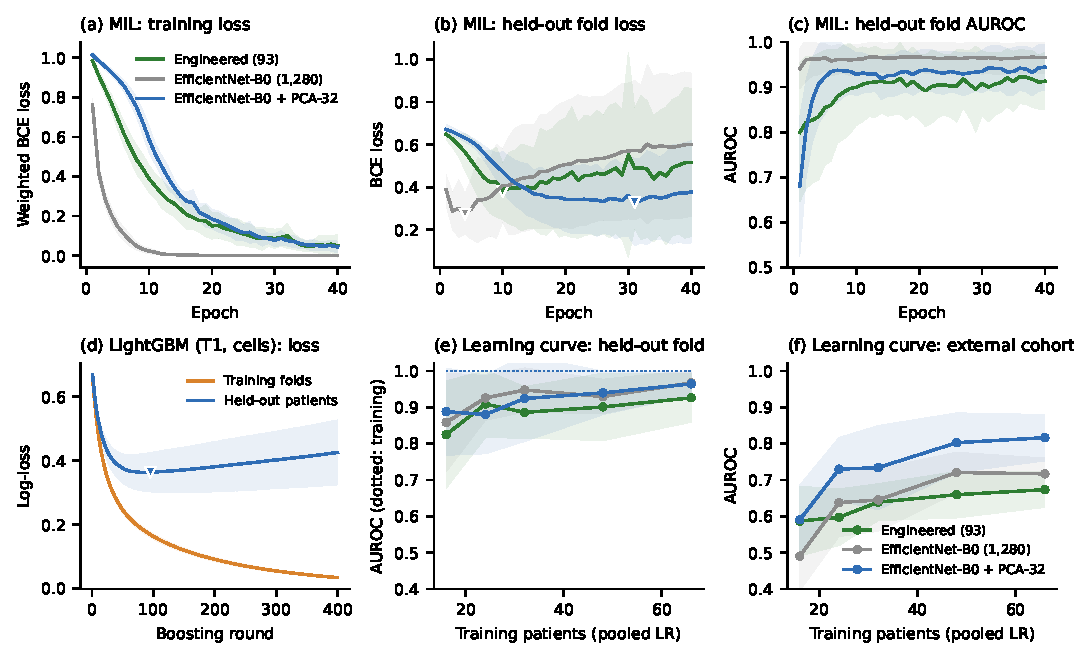
\includegraphics[width=\textwidth]{fig_training.pdf}
\caption{Training dynamics on the Discovery cohort (mean $\pm$ SD over 5 folds $\times$ 3 seeds). (a)--(c) Gated attention MIL trained with AdamW at a constant learning rate of $2\times10^{-4}$: training loss (class-weighted binary cross-entropy), loss and AUROC on the held-out fold per epoch; triangles mark the epoch with the lowest held-out loss. (d) Cell-level LightGBM for T1 (learning rate 0.05): log-loss on training folds and on held-out patients per boosting round. (e), (f) Learning curves of the pooled patient model versus the number of training patients, on the held-out fold (dotted: training AUROC) and on the external cohort. Values in (e) and (f) are for single fold models, not the fold ensemble used in the tables, and are therefore slightly lower.}
\label{fig:training}
\end{figure}

\section*{S5. Patient-level models without feature engineering}
\begin{table*}[!t]
\centering
\caption{Patient-level APL vs AML (T3). CV: Discovery, mean $\pm$ SD of three seeds. External: Validation cohort (24 patients), 95\% CI by patient bootstrap.}
\label{tab:patient}
\setlength{\tabcolsep}{2.5pt}
\begin{tabular}{llcccc}
\toprule
Features & Aggregation & CV AUROC & External AUROC [95\% CI] & Sens./Spec. & ECE \\
\midrule
Engineered & Pooled + LR & 0.867$\pm$0.059 & 0.674 [0.440, 0.896] & 0.67/0.58 & 0.380 \\
EfficientNet-B0 & Pooled + LR & 0.909$\pm$0.018 & 0.639 [0.412, 0.857] & 0.75/0.50 & 0.304 \\
Fusion & Pooled + LR & 0.910$\pm$0.018 & 0.667 [0.443, 0.874] & 0.50/0.67 & 0.319 \\
Engineered & Attention MIL & 0.827$\pm$0.003 & \textbf{0.778 [0.566, 0.943]} & 0.75/0.75 & 0.300 \\
EfficientNet-B0 & Attention MIL & 0.885$\pm$0.021 & 0.625 [0.385, 0.844] & 0.58/0.58 & 0.231 \\
Fusion & Attention MIL & 0.886$\pm$0.039 & 0.674 [0.437, 0.881] & 0.58/0.58 & 0.274 \\
\bottomrule
\end{tabular}
\end{table*}
\begin{figure}[!htbp]
\centering
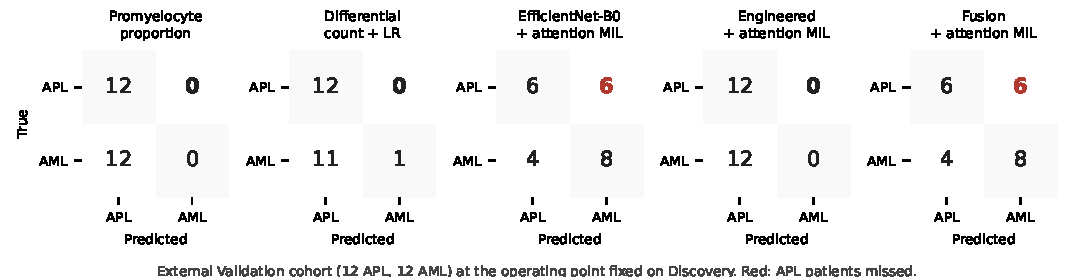
\includegraphics[width=\textwidth]{fig_confusion.pdf}
\caption{Confusion matrices on the external cohort at the operating point fixed on Discovery for a sensitivity of at least 0.95. Missed APL patients are shown in red.}
\label{fig:confusion}
\end{figure}

\section*{S6. Pooled 106-patient analysis and local recalibration}
\begin{table}[!t]
\centering
\caption{Secondary analysis with more statistical power: repeated (3$\times$) 5-fold patient-level CV over all 106 APL-AML patients. This is an internal analysis, not an external validation. $\Delta$: AUROC difference vs.\ the unreduced EfficientNet-B0 embedding (paired patient bootstrap on repeat-averaged scores). Recall, specificity and F1 at a threshold chosen for sensitivity $\ge0.95$ inside each training fold.}
\label{tab:pooled}
\setlength{\tabcolsep}{2.5pt}
\resizebox{\columnwidth}{!}{%
\begin{tabular}{lccccc}
\toprule
Model & AUROC [95\% CI] & $\Delta$ vs.\ no PCA & Recall (missed/34) & Spec. & F1 \\
\midrule
Promyelocyte fraction (biomarker) & 0.677 [0.572, 0.784] & -0.275*$^{\dagger}$ & 1.00 (0.0) & 0.00 & 0.49 \\
Engineered, pooled LR & 0.893 [0.823, 0.949] & -0.059* & 0.94 (2.0) & 0.42 & 0.59 \\
EfficientNet-B0, no PCA & 0.953 [0.898, 0.989] & -- & 0.95 (1.7) & 0.53 & 0.64 \\
EfficientNet-B0 + PCA-16 & 0.878 [0.802, 0.941] & -0.074*$^{\dagger}$ & 0.98 (0.7) & 0.35 & 0.58 \\
EfficientNet-B0 + PCA-32 & 0.947 [0.897, 0.985] & -0.005 & 0.96 (1.3) & 0.60 & 0.69 \\
EfficientNet-B0 + PCA-64 & 0.942 [0.892, 0.979] & -0.011 & 0.95 (1.7) & 0.63 & 0.70 \\
Engineered + PCA-32 fusion & 0.922 [0.853, 0.973] & -0.030 & 0.95 (1.7) & 0.58 & 0.67 \\
Engineered, attention MIL & 0.867 [0.794, 0.931] & -0.086* & 0.89 (3.7) & 0.52 & 0.62 \\
EfficientNet-B0, no PCA$^{\ddagger}$ & 0.929 [0.870, 0.974] & -- & 0.96 (1.3) & 0.48 & 0.63 \\
EfficientNet-B0 + PCA-16$^{\ddagger}$ & 0.872 [0.791, 0.939] & -0.057* & 0.96 (1.3) & 0.31 & 0.56 \\
EfficientNet-B0 + PCA-32$^{\ddagger}$ & 0.929 [0.866, 0.976] & +0.000 & 0.96 (1.3) & 0.46 & 0.62 \\
EfficientNet-B0 + PCA-64$^{\ddagger}$ & 0.935 [0.876, 0.979] & +0.006 & 0.97 (1.0) & 0.49 & 0.63 \\
\bottomrule
\multicolumn{6}{l}{\footnotesize * $p<0.05$ unadjusted; $^{\dagger}$ after Holm correction. $^{\ddagger}$ PCA scores at natural scale; $\Delta$ vs.\ no PCA with the same scaling.}
\end{tabular}}
\end{table}
\begin{table*}[!t]
\centering
\caption{Can a new laboratory restore the operating point with a few local cases? $k$ confirmed local patients ($k/2$ APL, $k/2$ AML) are drawn from the Validation cohort and the remaining $24-k$ patients are scored (2,000 random draws). R0: development threshold. R2: development threshold lowered, if needed, to just below the lowest score of the local APL cases. P(miss): probability that at least one APL patient in the test set is missed.}
\label{tab:recal}
\setlength{\tabcolsep}{3pt}
\resizebox{\textwidth}{!}{%
\begin{tabular}{lcccccccccccc}
\toprule
 & \multicolumn{4}{c}{R0, $k=0$} & \multicolumn{4}{c}{R2, $k=4$} & \multicolumn{4}{c}{R2, $k=8$} \\
\cmidrule(lr){2-5}\cmidrule(lr){6-9}\cmidrule(lr){10-13}
Model & Recall & Spec. & F1 & P(miss) & Recall & Spec. & F1 & P(miss) & Recall & Spec. & F1 & P(miss) \\
\midrule
EfficientNet-B0, no PCA & 0.50 & 0.67 & 0.55 & 1.00 & 0.69 & 0.56 & 0.63 & 0.84 & 0.80 & 0.49 & 0.68 & 0.68 \\
EfficientNet-B0 + PCA-64 (pre-decl.) & 0.50 & 0.92 & 0.63 & 1.00 & 0.70 & 0.66 & 0.68 & 0.82 & 0.80 & 0.44 & 0.68 & 0.66 \\
EfficientNet-B0 + PCA-16 & 0.92 & 0.67 & 0.81 & 1.00 & 0.92 & 0.62 & 0.80 & 0.83 & 0.92 & 0.58 & 0.79 & 0.67 \\
Engineered, attention MIL & 1.00 & 0.00 & 0.67 & 0.00 & 1.00 & 0.00 & 0.67 & 0.00 & 1.00 & 0.00 & 0.67 & 0.00 \\
Fine-tuned EfficientNet-B0 & 0.83 & 0.67 & 0.77 & 1.00 & 0.85 & 0.63 & 0.76 & 0.84 & 0.86 & 0.59 & 0.76 & 0.67 \\
\bottomrule
\end{tabular}}
\end{table*}

\section*{S7. Ablation of engineered feature groups}
\begin{table}[!t]
\centering
\caption{Feature-group ablation on the external cohort (engineered features, LR). $\Delta$: change in AUROC relative to all 93 features, paired patient bootstrap.}
\label{tab:ablation}
\resizebox{\columnwidth}{!}{%
\begin{tabular}{lcccc}
\toprule
 & \multicolumn{2}{c}{T2 Blast detection} & \multicolumn{2}{c}{T1 Diagnosis on cells} \\
\cmidrule(lr){2-3}\cmidrule(lr){4-5}
Setting ($n$) & AUROC & $\Delta$ [95\% CI] & AUROC & $\Delta$ [95\% CI] \\
\midrule
All features (93) & 0.950 & -- & 0.671 & -- \\
\midrule \multicolumn{5}{l}{\emph{Without one group}} \\
\quad Nuclear shape (84) & 0.949 & -0.001 [-0.003, +0.001] & 0.681 & +0.010 [-0.004, +0.024] \\
\quad Basophilic region (83) & 0.945 & -0.005 [-0.009, -0.003]* & 0.665 & -0.005 [-0.025, +0.010] \\
\quad Stain and colour (67) & 0.916 & -0.034 [-0.060, -0.015]* & 0.548 & -0.123 [-0.272, +0.046] \\
\quad Chromatin texture (77) & 0.939 & -0.012 [-0.023, -0.004]* & 0.675 & +0.004 [-0.007, +0.016] \\
\quad Local binary patterns (65) & 0.947 & -0.004 [-0.010, +0.002] & 0.670 & -0.001 [-0.019, +0.020] \\
\quad Nucleoli and granules (89) & 0.951 & +0.001 [-0.002, +0.004] & 0.671 & +0.000 [-0.006, +0.006] \\
\midrule \multicolumn{5}{l}{\emph{One group only}} \\
\quad Nuclear shape (9) & 0.810 & -0.140 [-0.212, -0.082]* & 0.549 & -0.121 [-0.283, +0.062] \\
\quad Basophilic region (10) & 0.823 & -0.127 [-0.198, -0.069]* & 0.579 & -0.092 [-0.242, +0.073] \\
\quad Stain and colour (26) & 0.912 & -0.038 [-0.078, -0.013]* & 0.682 & +0.011 [-0.032, +0.041] \\
\quad Chromatin texture (16) & 0.802 & -0.148 [-0.221, -0.086]* & 0.526 & -0.145 [-0.331, +0.067] \\
\quad Local binary patterns (28) & 0.793 & -0.157 [-0.225, -0.098]* & 0.581 & -0.090 [-0.241, +0.081] \\
\quad Nucleoli and granules (4) & 0.860 & -0.090 [-0.142, -0.054]* & 0.500 & -0.171 [-0.365, +0.057] \\
\bottomrule
\multicolumn{5}{l}{\footnotesize * $p<0.05$.}
\end{tabular}}
\end{table}
\begin{figure}[!htbp]
\centering
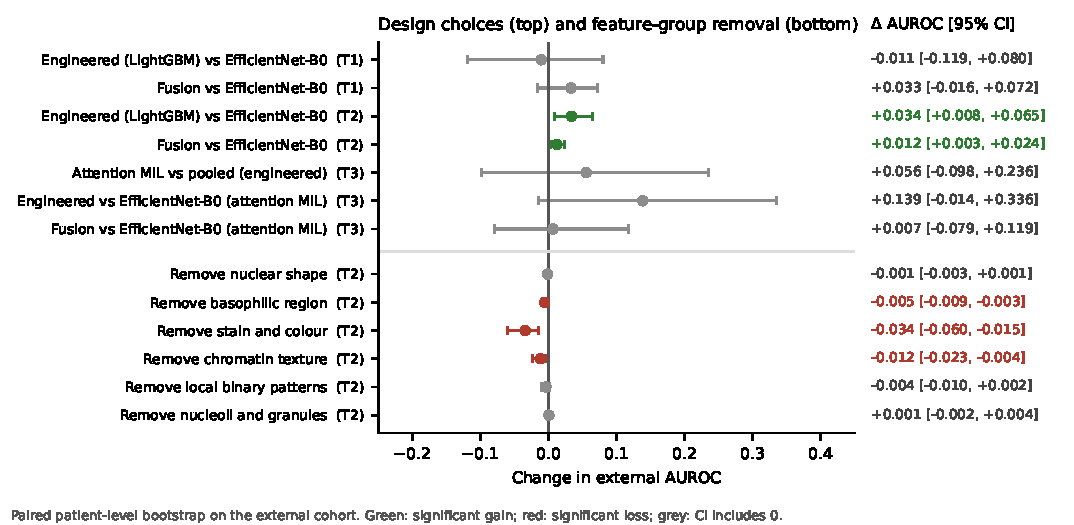
\includegraphics[width=\textwidth]{fig_impact.pdf}
\caption{Effect of design choices (top) and of removing each engineered feature group for blast detection (bottom) on external AUROC. Bars are 95\% confidence intervals from a paired patient-level bootstrap.}
\label{fig:impact}
\end{figure}

\bibliographystyle{IEEEtran}
\bibliography{refs}
\end{document}
